\nicebox{
Change your exercise structure so that instead of authentication with a static key, you implement this with certificates that you should create with openssl (PKI: xca).
}

A certification authority (CA) has to be created first in xca. For this we set the template to ca and pressed apply all extensions so that the final certificate will get the correct extensions.

Then fill all the fields under Subject, generate a new RSA key, and change the time range to 10 years, so that the certificate is valid for a long time.

\begin{figure}[H]
	\centering
	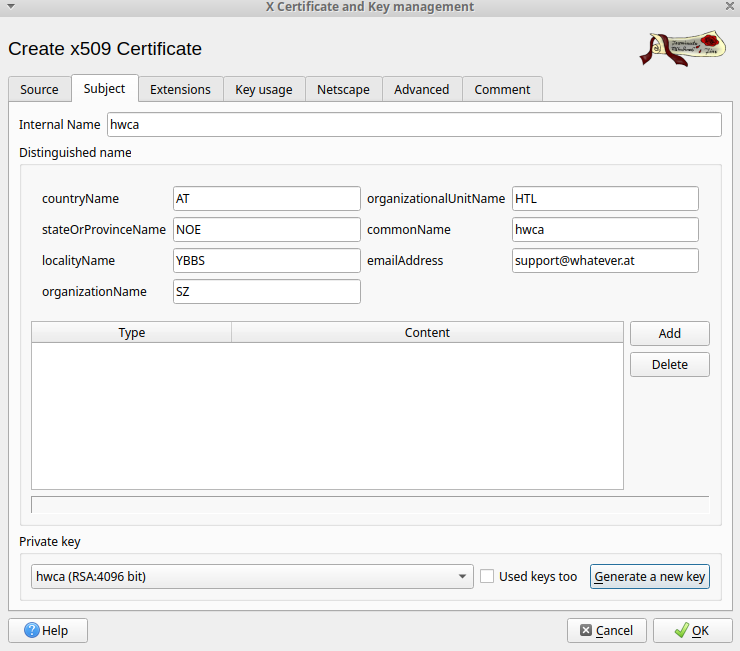
\includegraphics[width=0.8\linewidth]{Figures/create-ca.png}
	\caption{Creating a CA in xca}
\end{figure}

For creating the server and client certificates, we set the template to server and client respectively, use the ca we created before for signing and set the subject.

Then export the client and server certificates as a PKCS\#12 file, so that the private key is also included. Then transfer the files to the respective computers.

We also need diffie-hellman parameters, which can be generated under Extra -> Generate DH Parameters, these are only needed on the server side.

The new configuration for the home computer looks like this:

\begin{minted}{text}
dev tun0
proto udp
ifconfig 10.8.0.2 10.8.0.1
remote 192.168.60.1 1194
pkcs12 keys/hwclient.pfx
route 192.168.90.0 255.255.255.0 10.8.0.1
cipher AES-256-CBC
tls-client
\end{minted}

And for the office computer:

\begin{minted}{text}
dev tun0
proto udp
ifconfig 10.8.0.1 10.8.0.2
pkcs12 keys/hwserver.pfx
dh keys/dh2048.pem
port 1194
cipher AES-256-CBC
tls-server
\end{minted}

TLS has to be enabled on both sides, for certificates to be used. The certificates are then used in the pkcs12 directive, which includes the private key, certificate, and CA certificate.

This is the entire connection buildup using certificates from the server side:

\begin{minted}{console}
root@ntsi:/etc/openvpn\# openvpn --config office2.conf 2024-12-29 21:14:
58 OpenVPN 2.6.9 x86\_64-pc-linux-gnu [SSL (OpenSSL)] [LZO] [LZ4] [EPOLL]
[PKCS11] [MH/PKTINFO] [AEAD] [DCO] 2024-12-29 21:14:58 library versions:
OpenSSL 3.0.13 30 Jan 2024, LZO 2.10 2024-12-29 21:14:58 DCO version: N/A
Enter Private Key Password:

2024-12-29 21:15:00 WARNING: this configuration may cache passwords in
memory --- use the auth-nocache option to prevent this 2024-12-29 21:15:00
TUN/TAP device tun0 opened 2024-12-29 21:15:00 net\_iface\_mtu\_set: mtu
1500 for tun0 2024-12-29 21:15:00 net\_iface\_up: set tun0 up 2024-12-29 21:
15:00 net\_addr\_ptp\_v4\_add: 10.8.0.1 peer 10.8.0.2 dev tun0 2024-12-29 21:
15:00 Could not determine IPv4/IPv6 protocol. Using AF\_INET 2024-12-29 21:
15:00 UDPv4 link local (bound): [AF\_INET][undef]:1194 2024-12-29 21:15:00
UDPv4 link remote: [AF\_UNSPEC] 2024-12-29 21:15:04 peer info:
IV\_CIPHERS=AES-256-GCM:AES-128-GCM:CHACHA20-POLY1305 2024-12-29 21:15:04
peer info: IV\_PROTO=746 2024-12-29 21:15:04 [hwclient] Peer Connection
Initiated with [AF\_INET]192.168.60.2:1194 2024-12-29 21:15:05
Initialization Sequence Completed
\end{minted}